\scanpage{34}
% @ 1
\[
 \unsure{\mathbb{V}|V}(M)=\operatorname{Hom}_{k\text{-mod}}(M,k')
 =\operatorname{Hom}_{k'\text{-mod}}(M\otimes_k k',k')
\]
% @ 2
\uline{\unsure{tjrs|tjrs.}} représentable par
\[
 \operatorname{Sym}^{*}_k(M)=\sum_{n\geq0}\operatorname{Sym}^{n}_k(M)
\]

% @ 3–6
\[
\resizebox{\linewidth}{!}{\(\displaystyle\begin{aligned}
\Big[\, V(M)\times W(M)&\longrightarrow\deleted{\unsure{\mathbb{E}|E}}\unsure{\mathcal{O}|\mathscr{O}}_k=W(k)
&
\mathbb{V}(M)&\xrightarrow{\sim}
 \underbrace{\underline{\operatorname{Hom}}_{\mathcal{O}_k}
 (W(M),\deleted{\unsure{\mathcal{O}_k|\mathbb E_k}}W(k))}\\
&\unsure{V|\surd}&&
 k'\longmapsto\operatorname{Hom}\big(
  \overbrace{W(M)_{k'}}^{\inserted{\simeq\,W(\unsure{M_{k'}|M})}},
  \deleted{\unsure{\mathcal{O}_{k'}|\mathcal{O}_{k}}}W(k')\big)\\
&&&\hspace{3.7em}\vcenter{\hbox{\tikz[baseline]\node[rotate=90,inner sep=0pt]{\(=\)};}}\\[-.5ex]
&&&\operatorname{Hom}_{k'}(M_{k'},k')=\operatorname{Hom}_k(M,k'\unsure{)}
\end{aligned}\)}
\]

% @ 6–7
\unsure{Or|or}\quad $M\longmapsto W(M)$
\[
 \operatorname{Mod}(k)\longmapsto\operatorname{Mod}(\mathcal{O}_k)
 \qquad\text{est pl\uline{einement fidèle}.}
\]
% @ 8–10
\figure{\footnotesize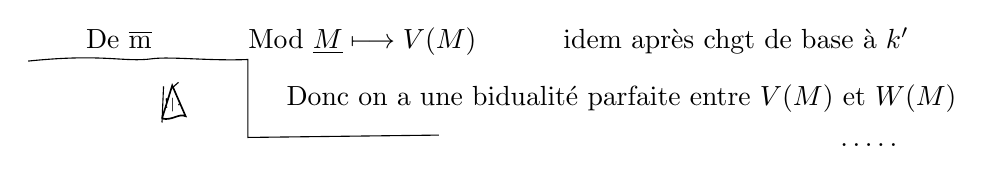
\begin{tikzpicture}[x=\linewidth,y=1cm]
\node[anchor=base west,inner sep=0pt] at (.06,1.18) {De $\overline{\mathrm{m}}$};
\node[anchor=base west,inner sep=0pt] at (.23,1.18) {\deleted{Mod} $\underline{M}\longmapsto V(M)$};
\node[anchor=base west,inner sep=0pt] at (.56,1.18) {idem après chgt de base à $k'$};
\draw (0,1.02) .. controls (.08,1.12) and (.10,1.00) .. (.13,1.05)
 .. controls (.15,1.08) and (.19,1.02) .. (.23,1.04)
 -- (.23,.05) -- (.43,.08);
\begin{scope}[shift={(.15,.45)},x=1cm,y=1cm]
 \draw[line width=.6pt] (-.12,-.16) -- (.01,.26) -- (.18,-.13)
  .. controls (.09,-.09) and (.01,-.19) .. (-.12,-.16);
 \draw (-.10,.25) -- (-.12,-.21) (.01,.23) -- (.09,.30);
 \node[inner sep=0pt] at (.02,.01) {\tiny\(\unsure{!|\cdot}\)};
\end{scope}
\node[anchor=base west,inner sep=0pt] at (.27,.46)
 {Donc on a une bidualité parfaite entre $V(M)$ et $W(M)$};
\node[anchor=base west,inner sep=0pt] at (.85,-.07) {.\,.\,.\,.\,.};
\end{tikzpicture}}

% @ 11
\[
 \underline{\operatorname{Aut}}_{\mathcal{O}}(M)\subset
 \underline{\operatorname{End}}_{\mathcal{O}}(M)
 \qquad\text{représentable si $M$ est proj., \unsure{t f.|t.f.}}
\]

% @ 12
\noindent\hspace{.05\linewidth}\rule{.31\linewidth}{.4pt}

% @ 13
\[
 \mu_n,\ D(\unsure{\vcenter{\hbox{\tikz[x=1ex,y=1ex]{\draw[line width=.12ex,line cap=round,line join=round] (0,0)--(.04,1.07)--(.94,1.09)--(.91,.6);\fill (.30,.82) circle[radius=.055ex];}}}|\Gamma|\Pi})\quad .\,.\,.
\]

% archive sheet number: 33
